\subsection*{The Important Questions}
The greetings card market is hundreds of years old and very well established. However, as society increasingly turns towards online solutions for it's problems, there have been new innovations in the greeting cards market --- we believe our service fits into this category. This leads to the following key question: ``Is there a space in the market for our service?''

For our market validation to be as relevant as possible, we must consider points raised by our Needs Analysis. We must dertermine whether or not our target audience gets a sense of social belonging, emotional value and esteem from sending and receiving greetings cards. This gives us the key question: ``How much value do consumers place on the emotional meaning behind a card?

Our Needs Analysis also mentions the functional values that our service could fulfil, that is, the effort that consumers must go through to remember an occasion and obtain a card to send. This leads to our final pair of questions: ``How much time do the consumers invest in acquiring a card?'' and ``Would consumers pay to have that need fulfilled with little to no effort?''

\subsection*{Secondary Research}
While market research suggests that global sales of greetings cards are declining \citep{strategyr}, our target market in the UK is actually growing at a significant rate \citep{greetingcardassociation}. For example in the UK, the value of the everyday cards market, such as birthday and anniversary cards, increased by \pounds28.7m to \pounds1.178bn in 2016 \citep{greetingcardassociation}. This growth matches a historical trend, with the UK greetings card market as a whole seeing a growth of \pounds28m in 2015 \citep{mintel}.

This market research carried out by Global Industry Analysis, Inc., the UK Greeting Card Association and Mintel is reflected in data obtained from Google Trends. Figure~\ref{fig:google_trends} shows search interest in ``birthday cards'' from January 2004 until March 2018 with the location restricted to the UK \citep{google_trends}.

  \begin{figure}
    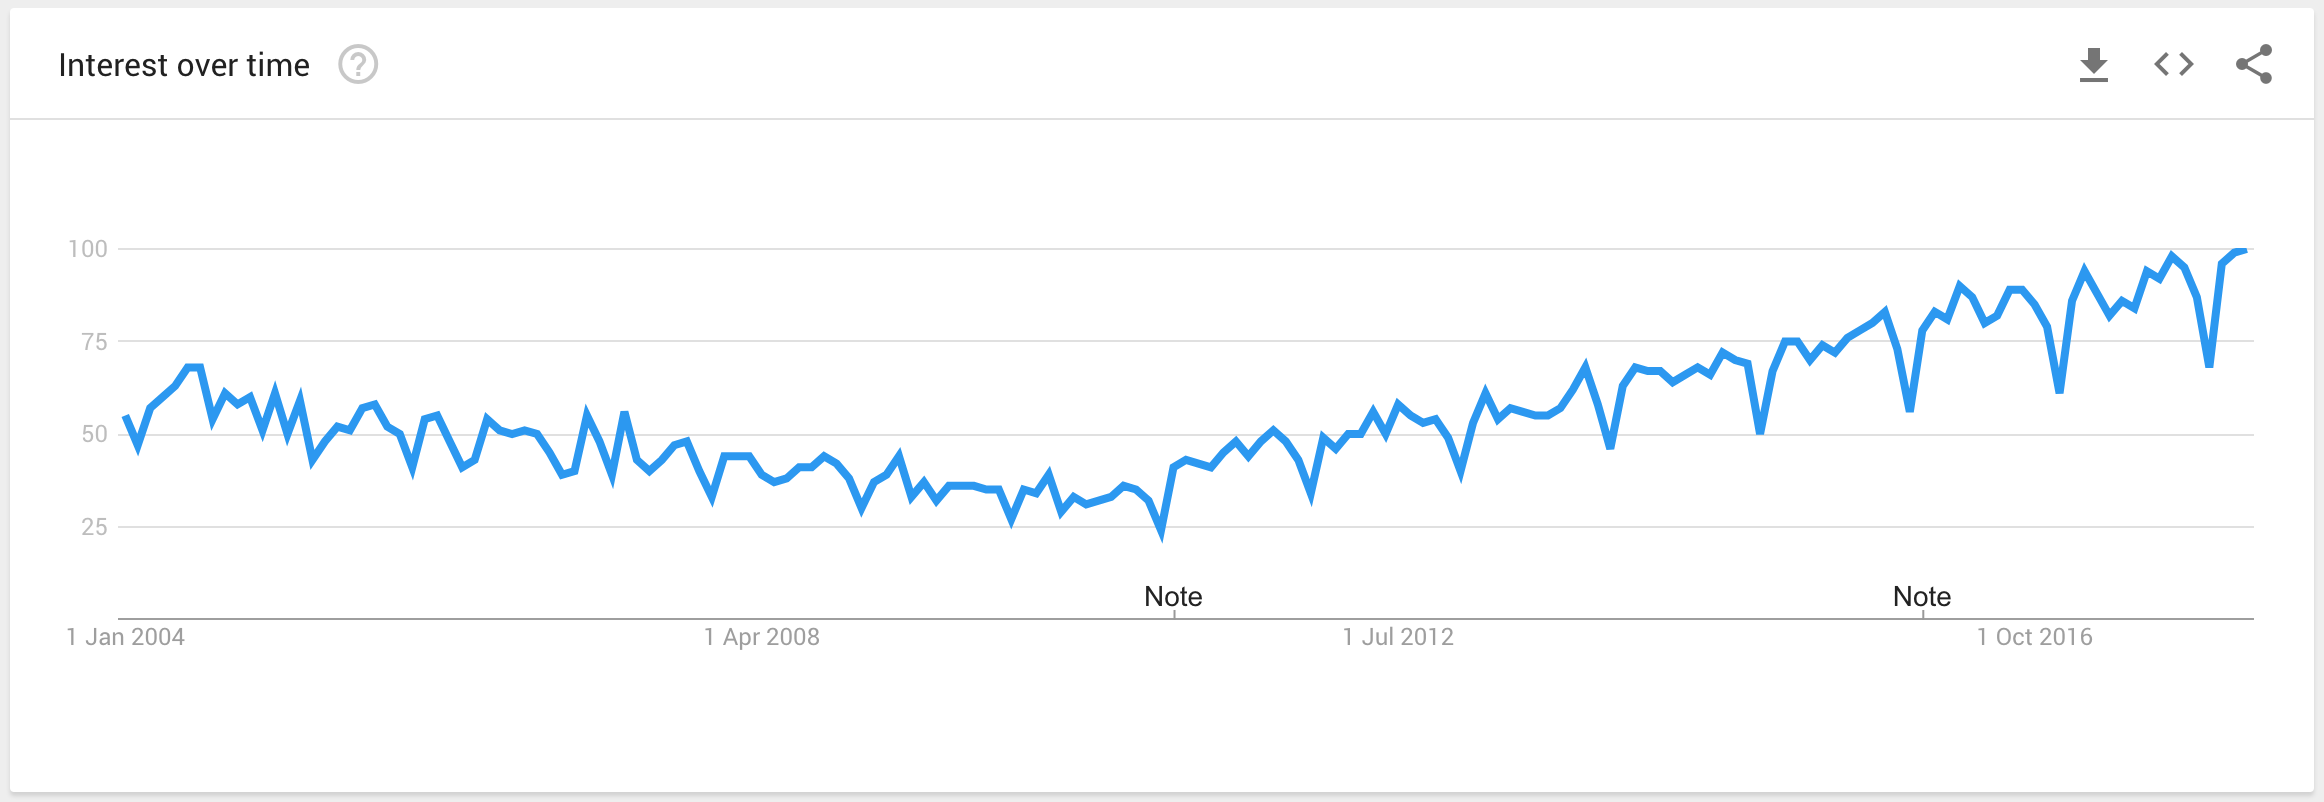
\includegraphics[width=\textwidth]{birthday_cards_google_trends.png}
    \caption{Google Trends result for 'Birthday Card' from 2004 - present in the United Kingdom}
    \label{fig:google_trends}
  \end{figure}

Google Trends allows us to see the most recent information on the interest a market. From this, it is evident that interest in greetings cards in the UK continued to increase throughout 2017 and into 2018. There are no signs that this increase is slowing, and as a result there is plenty of space in the market for new innovations that increase the accessibility of cards to consumers.

This growth is unsurprising, as the UK is already a significant part of the global greeting cards market. The UK market is the largest in Europe \citep{strategyr}, and sells more cards per capita than anywhere else, at 33 cards per person per year \citep{greetingcardassociation}. It is suggested that this is because sending and receiving cards is an important part of culture in the UK \citep{greetingcardassociation}.

The biggest area of competition for this product will be online; the decline of the greetings card industry elsewhere is attributed to the ease of sending a greetings message over the internet \citep{npr}. While this is noted as a threat to the UK industry, it has not had as large an impact as it has in other countries\citep{mintel}. Our goal is to introduce a service that is equally easy as sending a message online, but also retains the meaning and thoughtfulness behind traditional card giving.

There have been multiple startups, especially in the United States, that focus on the meaningfulness aspect. For example, Lovepop, a manufacturer of three dimensional pop-up cards received financial backing on the TV show Shark Tank \citep{americaninno} and has since seen success from selling their high-end cards through Etsy \citep{Etsy}. It is premium cards similar to these that we plan to use as they are more special and unexpected.

In the UK, a notable startup is Moonpig, an online service that delivers personalised cards directly to the recipient. They have continued to grow since their \pounds120m acquisition by PhotoBox \citep{bbc}. While Moonpig and its competitor Funky Pigeon are successful, market research still suggests that online card sales are lagging behind sales from physical stores \citep{mintel}, meaning there is room for innovation in this area.

\subsection*{Primary Research}
We wanted to get feedback on our idea early on, before we had invested too much time and effort into it, but struggled to find any experts in the greetings card industry. Instead, we focussed on approaching people who may want to use our service, and people who may be likely to receive cards delivered through our service. We decided to interview a range of these people rather than using questionnaires; interviews enabled us to get a more detailed and personal exploration of the interviewee's needs, as we could ask them to elaborate if we didn't understand anything they said, or probe for more information.

Before asking individuals specifically about our service, we firstly asked them more general questions in order to gain a firmer understanding about how they send greetings cards and how they feel about receiving them. This enabled us to refine our business idea based on their feedback, before carrying out a second round of interviews focussed on finding their thoughts about our refined idea.

For the first round of interviews, we used a set list of questions which consisted of the important questions that we had discovered from part A, and also from analysing the user needs we had previously ascertained. We interviewed a total of eight people, and conducted the majority of the interviews in person. Some of the interviewees were students, and some were working adults. The full interview results are included in the appendix, and some relevant key findings are listed below:

\begin{itemize}
  \item There was a mixed response on whether or not people struggle to remember to send greeting cards
  \item Nearly everyone said that they remember birthdays and important dates without the aid of any physical or virtual tools
  \item Five out of eight of the interviewees said that the quality of a card is important
  \item The majority of interviewees preferred to receive a card with a handwritten message inside, rather than a personalised, printed one
\end{itemize}

The first and second points consolidate our hypothesis that an automated card sending service may be useful for some people, but not so much for others. Upon hearing that five of the eight interviewees felt that the quality of a card is important, we decided to focus our service on luxury greetings cards, rather than budget ones. Originally we had thought that the service could print the message inside the card in a cursive font and send it directly to the recipient, but after hearing that people generally preferred to receive a handwritten card than a printed personalised message, we chose to not include that feature. We now envision that a blank card will be sent to the customer along with the envelope complete with the recipient's address and a prepaid stamp, so that they can write their message inside the card and mail it to the recipient.

Next, we created some new interview questions designed to find out how people felt about our newly refined business idea. We interviewed three people who had previously mentioned that they find it hard to remember to send cards and care about the quality of cards, as this would be our target audience. Again, the interviewees were a mixture of students and working adults. Full results are in the appendix and below are some key findings:

\begin{itemize}
  \item People expressed interest in the idea of an automated card sending service
  \item People expressed interest in the idea of receiving an envelope with the recipient's address and a prepaid stamp and a card which they can hand write and send themselves, presumably as this wouldn't be too much effort and would be more personal
  \item One interviewee mentioned that they would like to be able to choose the category of card to be sent
\end{itemize}

The results are positive and suggest that our idea has potential, however we are aware that we may be a victim of the ``Mom Test''. To combat this, we asked questions such as ``would you prefer a system which offers x or y'', rather than ``how do you feel about a system offering x''. This did make it harder to gain results specifically about our business idea, and we are also aware that the results we did find may have been influenced by a social bias, as we had interviewed friends and family.

Therefore, for to gain further and more concise market validation, we have planned to create and launch a prototype website where customers can sign up to our service, and analyse it to discover whether there is in fact a market for our idea. If we were properly launching our business, we would need a partner greetings cards firm to create the cards for us and send them to the customers. However, we want to find out whether people would use our system before investing too much time into it. Therefore we plan to manually buy and send the cards to customers ourselves. This will be the next step we are planning to take.

\subsection*{Competitors}
Our main competitors fall into three categories. Firstly, there are the card shops or supermarkets selling greeting cards, such as Sainsbury's and CardFactory. We aim to differentiate our business firstly by offering convenience --- customers do not have to go to a shop to buy a card. Secondly, our service is automated, meaning that customers do not have to actively try to remember their contacts' meaningful dates. Customers enter the dates into Natalis and are notified by email when the date is draws near.  Finally, our service will offer high end greetings cards, whereas these shops generally offer cards towards the lower end of the market. Although these companies are successful, these differences should ensure that our company will not be in direct competition with them.

The next group of competitors we will face are online greetings card companies, such as MoonPig and Funky Pigeon. These businesses are well established within the market, therefore it is imperative that our value proposition differentiates Natalis from these incumbents..

Again, we will differentiate ourselves by providing an automated card sending service, and providing high end greeting cards. Specifically concerning these competitors, our service is unique in how the personal aspect of sending cards is maintained. Customers may still write the message inside the card, rather than having it printed by a computer, unlike the offerings of MoonPig and Funky Pigeon.

Finally, the last group of competitors will be e-commerce websites such as Etsy and Redbubble. These websites provide a platform for individual artists to sell a wide range of unique and handmade goods. We will differentiate ourselves from these competitors by focusing on the sale and distribution of handmade, quality greetings cards.

Table~\ref{table:competitor_analysis} directly compares the features of Natalis with the offerings of its competitors.

\begin{table}[h]\footnotesize\centering
 \begin{tabular}{ | p{2cm} | p{2cm} | p{2cm} | p{2cm} | p{2cm} | p{2cm} | }
    \hline
    Feature & Natalis & Supermarkets & CardFactory/ Clintons & Moonpig/ Funky Pigeon & Redbubble/ Etsy \\
    \hline
    Online & \cellcolor{tableGreen}Yes & \cellcolor{tableRed}No & \cellcolor{tableRed}No & \cellcolor{tableGreen}Yes & \cellcolor{tableGreen}Yes \\
    Card Specialist & \cellcolor{tableGreen}Yes & \cellcolor{tableRed}No & \cellcolor{tableGreen}Yes & \cellcolor{tableGreen}Yes & \cellcolor{tableRed}No \\
    Premium Cards& \cellcolor{tableGreen}Yes & \cellcolor{tableRed}No & \cellcolor{tableRed}No & \cellcolor{tableRed}No & \cellcolor{tableGreen}Yes \\
    Reminders & \cellcolor{tableGreen}Yes	& \cellcolor{tableRed}No & \cellcolor{tableRed}No & \cellcolor{tableRed}No & \cellcolor{tableRed}No \\
    \hline
  \end{tabular}
  \caption{Feature comparison between Natalis and its competitors.}
	\label{table:competitor_analysis}
\end{table}